\documentclass{article}
\usepackage{amsmath}
\usepackage{amssymb}
\usepackage{empheq}
\usepackage{graphicx}
\usepackage{subcaption}
\usepackage{booktabs}
\usepackage{geometry}
\usepackage{mathtools}
\usepackage{url}
\geometry{left=2.5cm,right=2.5cm,top=2.5cm,bottom=2.5cm}

\title{\textbf{Lecture Note} \\
		\large CS5339 Theory and Algorithm for Machine Learning}
\author{Meng-Jiun Chiou \\ National University of Singapore \\ mengjiun.chiou@u.nus.edu}
\date{}

\begin{document}
    \maketitle 
    \section{Supervised Learning}
    \subsection{Empirical Risk Minimization (ERM)}
    The learner does not know $D$ and only have access to the training set $S$, a sample from $D$. For a predictor $h: X \rightarrow Y$, we can approximate the expected error by using the training set error
    \begin{equation}
    L_S(h) = \frac{|i \in {1,...,m}:h(x_i) \neq y_i|}{m}.
    \end{equation}
    It can be rewritten using the 0-1 loss
    \begin{equation}
    L_S(h) = \frac{\sum_{i=1}^m l_{0-1}(h, (x_i, y_i))}{m}.
    \end{equation}
    Training set error is often called the empirical error or empirical risk. Given a hypothesis class $H$, finding the hypothesis $h \in H$ that minimizes the empirical risk is a simple learning strategy, which is often called empirical risk minimization (ERM).
    
    
    \subsection{Maximum Likelihood Estimation (MLE)}
    Assume that the data distribution $P$ is known up to some parameter $h \in H$, MLE selects the $h$ that maximizes the probability of the data $S$ being observed:
    \begin{equation}
    h_{ML} = \arg \max_{h\in H} P(S|h).
    \end{equation}
    For i.i.d. data $S = (z_1,...,z_m) \sim D^m$, this becomes:
    \begin{equation}
    h_{ML} = \arg \max_{h \in H} \prod_{i=1}^m D(z_i | h).
    \end{equation}
    For supervised learning, $z_i = (x_i, y_i)$ and we have
    \begin{align}
    h_{ML} &= \arg \max_{h \in H} \prod_{i=1}^m D(y_i | x_i, h) D(x_i) \\
    	   &= \arg \max_{h \in H} \prod_{i=1}^m D(y_i | x_i, h) \\
           &= \arg \max_{h \in H} \sum_{i=1}^m log D(y_i | x_i, h).
    \end{align}
    With an equivalent distribution can be found, empirical risk minmization (ERM) is equal to maximum likelihood when for loss function
    \begin{equation}
    l(h, (x,y)) = -\ln p(y|x,h).
    \end{equation}
    
    \subsection{Classification Loss Functions}
    For binary classification using $h(x) \in (-\infty , \infty)$, we often compose the output of our function $h(x)$ with the logistic (sigmoid) function to get a probability model 
    \begin{align}
    P(y=1|x,h) &= \frac{\exp(h(x))}{1 + \exp(h(x))} = \frac{1}{1+\exp(-h(x))} \\
    P(y=-1|x,h) &= 1-\frac{\exp(h(x))}{1 + exp(h(x))} = \frac{1}{1 + \exp(h(x))}.
    \end{align}
    For $y \in \{1,-1\}$, can write $P(y|x,h) = \frac{1}{1+\exp(-yh(x))}.$ Therefore log loss can be written as
    \begin{equation}
    l_{\log}(h,(x,y)) = -\log P(y|h(x)) = \log(1+\exp (-yh(x))).
    \end{equation}
    When $h(x)$ is a linear function, this is often called \textit{logistic regression}. \\\\
    For multi-class classification, 
    \begin{equation}
    P(y=k|x,h)=\frac{\exp(h_k(x))}{\sum_{i=1}^K \exp (h_i(x))}.
    \end{equation}
    When $h_i(x)$ is linear, it is often called \textit{multiclass logistic regression, softmax regression or maximum entropy classifier}.
    
    \subsection{Maximum A Posteriori Estimation (MAPE)}
    Instead of maximizing the likelihood, MAP find the parameter that maximizes the posterior probability $P(h|D)$:
    \begin{align}
    h_{MAP} &= \arg \max_{h \in H} P(h|D) \\
    		&= \arg \max_{h \in H} P(D|h)P(h) \\
            &= \arg \max_{h \in H} \prod_{i=1}^m D(z_i|h)P(h) \\
            &= \arg \max_{h \in H} \sum_{i=1}^m \Big( \log D(y_i|x_i, h) + \log P(h) \Big).
    \end{align}
    So balance between fitting the data (likelihood) and fitting the prior well. For example, we add an zero mean Gaussian prior on the weight vector $\lambda ||\textbf{w}||^2$ in loss function of linear regression. This is often called \textit{ridge regression} or penalized least square. Minimizing a combination of empirical risk and a regularizer is also called Regularized Risk Minimization (RRM).
    
    \subsection{Bayesian Estimation}
    Instead of selecting a single $h$, we maintain the posterior distribution over the parameters $P(h|z_1,...,z_m)$. This can be used to make optimal prediction (assuming the prior is correct) for the variable of interest. For example, 
    \begin{align}
    P(y|x,z_1,...,z_m) &= \int_h P(y,h|x,z_1,...,z_m) \\
    				   &= \int_h P(y|h,x,z_1,...,z_m) P(h|z_1,...,z_m).
    \end{align}
    
    
    \section{Unsupervised Learning}
    Many (but not all) unsupervised learning problems can be posed as density estimation problems, i.e. learning the distribution of the data. We can also pose the problem of learning the data distribution as a maximum likelihood (or maximum a posteriori) estimation problem. 
    \\\\
    For lossless compression, using $P(x_1,...,x_n)$ to compress $x_1,...,x_n$ using Hoffman coding or arithmetic coding, gives the  shortest code length of $-\sum_{i=1}^m \log P(x_i|h)$ (ignoring rounding required for discrete lengths). Therefore, maximizing $P(x_i|h)$ is equal to minimizing number of bits required.
    
    \section{Discriminative/Generative Models}
    The approach of directly optimizing for the loss that we are interested in is called \textbf{discriminative learning}. Another approach is to ignore the fact that the data for supervised learning comes in pairs $z=(x,y)$ and learn the data distribution (density estimation) for $z$. After we have learned a model for $p(z) = p(x,y)$, we perform inference to get our estimate of $y$ by computing $p(y|x)$. This approach is called \textbf{generative learning}. We illustrate this approach using two common learning models: naive Bayes and linear discriminant analysis (LDA).
    
   \subsection{Naive Bayes}
   The Bayes optimal classifier is 
   \begin{align}
   h_{Bayes}(x) &= \arg\max_{y \in {-1, 1}} P(Y=y|X=\textbf{x}) \\
   				&= \arg\max_{y \in {-1, 1}} P(Y=y)P(X=\textbf{x}|Y=y)/Z
   \end{align}
   and we make the naive generative assumption that, the features are independent of each other given the label, i.e.
   \begin{equation}
   P(X=\textbf{x}|Y=y) = \prod_{i=1}^d P(X_i=x_i|Y=y).
   \end{equation}
   Hence, the classifier becomes.
   \begin{align}
   h_{Bayes}(x) &= \arg\max_{y \in {-1, 1}} P(Y=y) \prod_{i=1}^d P(X_i=x_i|Y=y) \\
   &= \arg\max_{y \in {-1, 1}} \log P(Y=y) + \sum_{i=1}^d \log P(X_i=x_i|Y=y) \\
   &= sign(w_0 + \sum_{i=1}^d(w_{i,0}x_{i,0}+w{i,1}x{i,1})).
   \end{align}
   There comes a question: which is better, Naive Bayes or logistic regression? An answer \cite{4690} said it depends on the distribution of data. If the data set is large, discriminative model may perform better as it models directly $p(y|x)$. On the other hand, if there are some extra unlabeled data, generative model may do better as it can deal with missing data.
   
   \subsection{LDA}
   LDA and QDA classifiers are attractive because they have closed-form solutions that can be easily computed, are inherently multiclass, have proven to work well in practice and have no hyperparameters to tune. Linear Discriminant Analysis can only learn linear boundaries, while Quadratic Discriminant Analysis can learn quadratic boundaries and is therefore more flexible..
   
   \subsection{Discriminative VS Generative Classifiers}
   Here are some comparisons between these two classes of models. Pros for \textbf{discriminative models}:
   \begin{itemize}
   \item Discriminative classifiers are more robust against misspecification of the model, while generative classifiers depend on the model being correct. If the model is wrong, the discriminative model can still converge to the best approximation within the model class as the data size increases.
   \item It is usually easier to add features to discriminative models. For generative model, we need to try to find the correct model for the feature, which can be difficult.
   \end{itemize}
   Pros for \textbf{generative models}:
   \begin{itemize}
   \item It is sometimes computationally cheaper to train generative classifiers, e.g. Naive Bayes mostly requires only counting.
   \item It may converge faster, e.g. Naive Bayes converges faster than logistic regression.
   \item It handles missing and unlabeled training data naturally. In doing inference, they are marginalized away. However, in discriminative models there is no standard way for handling missing/unlabeled variables.
   \end{itemize}
   
   \section{Feature}
   \subsection{Filter}
   Asses each feature independently of other features. We may select $k$ features that achieves the highest score, using \textbf{Pearson correlation coefficient}:
   \begin{equation}
   \rho_(X_j, Y) = \frac{cov(X_j, Y)}{\sqrt{var(X_j)var(Y)}} = \frac{cov(X_j, Y)}{\sigma_{X_j} \sigma_{Y}}
   \end{equation}
   For classification, \textbf{mutual information} (MI) is often used. Not limited to real-valued random variables like the correlation coefficient, MI is more general and determines how similar the joint distribution $p(X,Y)$ is to the products of factored marginal distribution $p(X)p(Y)$. MI is defined as:
   \begin{align}
   I(X_i;Y) &= \sum_{x_i} \sum_{y} p(x_i, y) \log \frac{p(x_i, y}{p(x_i)p(y)} \\
   			&= H(Y) - H(Y|X),
   \end{align}
   where $p(x_i,y)$ is the joint probability function of $X$ and $Y$, and $p(x_i)$ and $p(y)$ are the marginal probability distribution functions of $X$ and $Y$ respectively and $H(Y) - H(Y|X)$ is the difference between the entropy of the label $Y$ and the conditional entropy of $Y$ given input $X$ and is also called the \textbf{information gain}. For feature selection, we rank features according to information gain, and select the $k$ features with the largest information gain. Another commonly used feature selection method is \textbf{chi square} which tests whether the feature is independent of the label.
   
   \subsection{Wrapper}
   Filter approaches do not take into account dependence among the features. Wrapper approaches search for subset of variables that will perform well. Common greedy methods include:
   \begin{itemize}
   \item Forward selection: Features are progressively added as learning is done. e.g. Viola-Jones face detector is trained using Adaboost.
   \item Backward elimination: Starting with all variables and progressively eliminate the least promising ones.
   \end{itemize}
   
   \subsection{Sparsity-Inducing Norms}
   We can formulate the feature selection problem as:
   \begin{equation}
   \min_{w} L_S(\textbf{w}) s.t. ||\textbf{w}||_0 \leq k,
   \end{equation}
   where $||\textbf{w}||_0 = |\{ i:w_i \neq 0 \}|.$ is also called $l0$ norm. As this is often computationally hard, so we often relax into $l1$ norm:
   \begin{equation}
   \min_{w} L_S(\textbf{w}) s.t. ||\textbf{w}||_1 \leq k,
   \end{equation}
   which can be solved efficiently if $L_S$ is convex (convex optimization problem). We can also encourage a sparse solution to use the $l1$ norm of the weight as a regularizer,
   \begin{equation}
   \min_{w} (L_S(\textbf{w}) + \lambda ||\textbf{w}||_1),
   \end{equation}
   which again is convex if $L_S$ is convex, e.g. in logistic regression. 
   \\\\
   We can derive Lasso as MAP with each $w_i$ independently distributed with Laplacian prior $Pr(w_i) = \frac{\lambda}{2}\exp(-\lambda |w_i|)$. Refer to Figure \ref{fig:lasso_ridge}.
   \begin{figure}[h!]
   \centering
   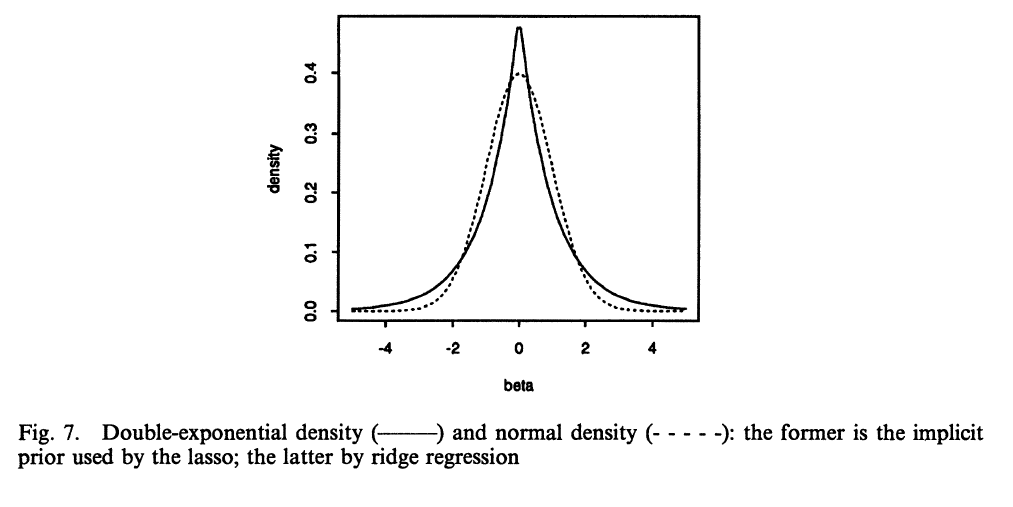
\includegraphics[width=.8\columnwidth]{lasso_ridge}
   \caption{Laplacian prior (l1, double-exponential density) versus Gaussian prior (l2, normal density).}
   \label{fig:lasso_ridge}
   \end{figure}
   Compared to Lasso, Ridge regression performs poor for the data out of range of training data. Lasso regression zeros out most of the coefficients.
   
   \subsection{Common Feature Transformation Methods}
   Let $\textbf{f} = (\text{f}_1,...,\text{f}_m) \in \mathbb{R}^m$ be the value of feature f over the $m$ training examples and $\bar{\text{f}} = \frac{1}{m} \sum_{i=1}^m \text{f}_i$.
   \begin{itemize}
   \item Centering
   \item Unit Range
   \item Standardization (zero mean and unit variance)
   \item Clipping
   \item Sigmoidal Transformation
   \item Logarithmic Transformation
   \end{itemize}
   
   \subsection{Feature Learning}
   
   
   \bibliographystyle{ieeetr}
   \bibliography{citations}
\end{document}